% =====================================================================
% Transportation Research Part C -- journal extension of the SID 2026
% paper (paper/sid2026). Class: elsarticle (Elsevier), author-year
% references (elsarticle-harv), single column, preprint layout.
%
% VERIFY BEFORE SUBMISSION (ScienceDirect blocks automated access, so
% the specifics below come from secondary sources dated 2026-08):
%   - abstract limit (~250 words), highlights file (3-5 bullets,
%     <=85 characters each), graphical abstract, CRediT, data
%     availability statement, declaration of competing interests,
%     generative-AI disclosure. See SUBMISSION_NOTES.md.
%
% The horizon section was filled on 2026-08-21 from
% studies/2026-08-trc-horizon/ tables (GPU run, exit 0). Every figure
% quoted is read from studies/2026-07-fuel-study/tables/, from
% studies/2026-08-trc-horizon/tables/, or from the SID paper.
%
% RE-BASELINED 2026-09-01: the original study archive was built before
% skyrank commit 7075cd3 keyed pair completeness on (pair_id,
% snapshot_date); pair_id is recycled across days, so ~25% of valid
% pairs had been silently dropped (225,181 -> 281,720 test pairs). The
% full study and the horizon experiment were re-run on the corrected
% archive and every number in this manuscript re-verified against the
% regenerated tables.
% =====================================================================
\documentclass[preprint,authoryear,12pt]{elsarticle}

\usepackage[T1]{fontenc}
\usepackage{booktabs}
\usepackage{graphicx}
\usepackage{amsmath}
\usepackage[hidelinks]{hyperref}
\graphicspath{{figures/}}

% the class's first-page footline ("Preprint submitted to <journal>
% <date>") is wider than the 390 pt text block with this journal's full
% name; same wording, one point smaller, so it fits the measure
\makeatletter
\def\ps@pprintTitle{%
  \let\@oddhead\@empty \let\@evenhead\@empty
  \def\@oddfoot{\fontsize{9}{11}\selectfont\itshape
    Preprint submitted to Transportation Research Part C%
    \hfill\enspace\today}%
  \let\@evenfoot\@oddfoot}
\makeatother

% loosen float placement so the figure queue cannot jam: elsarticle's
% defaults deferred the maps figure past the references
\renewcommand{\topfraction}{0.9}
\renewcommand{\textfraction}{0.05}
\renewcommand{\floatpagefraction}{0.75}
\setcounter{topnumber}{3}

\journal{Transportation Research Part C: Emerging Technologies}


% Typesetting: no single line of a paragraph may be stranded at the top or
% the bottom of a page or column, and no word may be hyphenated across a
% page break. These are the standard penalties; they cost a little vertical
% justification and buy pages that read continuously.
\clubpenalty=10000
\widowpenalty=10000
\displaywidowpenalty=10000
\brokenpenalty=10000

\begin{document}

\begin{frontmatter}

\title{Predicting airline acceptance of fuel-saving reroutes from
flight-plan revisions}

\author[ih]{Ramon Dalmau\corref{cor}}
\ead{ramon.dalmau-codina@eurocontrol.int}
\author[muac]{David Perez}
\author[ih]{Franck Ballerini}
\author[muac]{Seddik Belkoura}
\author[muac]{Vincent Taverniers}
\author[muac]{Gratiel Marius Marin}
\author[ih]{Robin Deransy}
\author[hq]{Benjamin Cramet}
\author[hq]{Grigori Gustin}
\cortext[cor]{Corresponding author.}
\affiliation[ih]{organization={EUROCONTROL Innovation Hub},
  city={Br\'etigny-sur-Orge}, country={France}}
\affiliation[muac]{organization={EUROCONTROL Maastricht Upper Area
  Control Centre}, city={Maastricht}, country={the Netherlands}}
\affiliation[hq]{organization={EUROCONTROL Headquarters},
  city={Brussels}, country={Belgium}}

% Cut for space 2026-09-06 (the abstract stood at 311 words against the
% 250 this project's own acceptance check requires; SUBMISSION_NOTES.md
% recorded 231 on 2026-09-04 and was stale). Removed, in order:
%   "That is a stronger record of preference than earlier work had, since
%    its alternatives were generated rather than filed and an airline may
%    never have seen them."
%   "A channel offering the cheaper route to every flight would therefore
%    be wrong more often than right, and" (the following clause was kept
%    and re-opened as "What a channel needs is therefore a way of ...")
%   "against the 44.9\,\% of proposing the cheaper route on every eligible
%    flight," (a comparator only the simulation's blindfold makes available)
%   "on the two extrapolation bases available"
% Redrafted 2026-09-09 at the author's request: the previous abstract
% "looks like random sentences... does not have flow... is not catchy."
% This version was checked against two fresh zero-context readers, who
% both flagged the same fix on the first draft handed to them: a
% sentence on model ageing, appended after the channel result, read as
% an unrelated result bolted onto the argument and, worse, produced two
% disconnected caveats back to back once the "never revise" limitation
% followed it. That sentence is cut; at the time this comment was
% written, ageing was still reported in full in the Introduction's
% contribution list and its own section, so nothing was lost from the
% paper, only from the abstract. The model-ageing section was itself
% cut in full on 2026-09-09 (see the comment above
% Section~\ref{sec:validity}), so this abstract cut is now moot but
% left as the record of what was actually checked. The
% "against 55.0\,\%" framing (not naming which single-indicator rule
% reaches it) and the single-basis fuel figure (dropping the CO$_2$
% annualisation range) follow the same "explain less" instruction and
% the 2026-09-08 political-sensitivity redaction described where this
% comment used to sit; both are unpacked in the body.
\begin{abstract}
Every flight-plan revision records a choice an airline actually made:
the route it dropped, and the route it filed instead. Eighteen months
of European air traffic hold 1.48 million such pairs, read here as
revealed preferences and used to train a ranking model that predicts,
between two candidate routes, which one an airline would choose.
Tested on data it never saw during training, the model identifies the
chosen route 68.1\,\% of the time, rising to 94.9\,\% on the fifth of
decisions it is most confident about. That confidence is calibrated,
so a proposal channel built on the model can offer a cheaper route
only when acceptance is likely, at a precision fixed in advance.
Simulated against what the airlines actually filed next, such a
channel reaches 79.2\,\% precision and surfaces tens of kilotonnes of
planned-fuel savings a quarter. Its clearest blind spot is the flights
that never revise at all, though a much scarcer set of matched pairs
closes most of that gap. Airline route acceptance, this paper shows,
is learnable from records the network already keeps.
\end{abstract}

\begin{keyword}
air traffic flow management \sep airline preferences \sep learning to
rank \sep fuel efficiency
\end{keyword}

\end{frontmatter}

% =====================================================================
\section{Introduction}
\label{sec:intro}

On a spring morning in 2026, an Airbus A320 was filed from Amsterdam to
Barcelona on a route carrying 102 minutes of attributed air traffic
flow management (ATFM) delay, and the airline subsequently re-filed.
The new route shed that delay completely, and it cost the airline on
each of the three counts an airline pays for directly: 39 minutes of
flight time, 1\,397\,kg of extra planned fuel, and 466 euros more in
en-route charges. Both routes are held in the network's records and so,
implicitly, is the airline's judgement that the delay would have cost it
more than the detour did.
% CORRECTED 2026-09-07: the paragraph listed what the detour cost but
% omitted en-route charges, the third of the three costs the paper uses
% throughout. Verified for this pair in
% data/ich_dataset/ich_dataset_2026-05.parquet, pair_id 1421263:
% kpiRouteChargeIndicator 1274 -> 1740 EUR (units per run_01_eda.py:41).

That judgement is the quantity this paper models. A flight plan is not
filed once and left alone: an airline may revise it at any time until
the aircraft leaves, and the network's response is only one of the
reasons for doing so. Attributed delay of the kind the opening flight
was carrying is the most visible prompt; an aircraft arriving late from
its previous leg is another, since the delay it brings consumes the
slack the rotation was holding, and an updated forecast is a third,
since changed winds change the time and fuel every candidate route
would need. A route may also simply cease to be filable, in which case
the revision is not a choice at all. What the archive records is what
changed rather than why, and it does not separate one reason from
another; every revision nonetheless leaves the same trace, the route
replaced and the route that replaced it, and therefore a preference
the airline expressed with its own filing system rather than in
answer to a survey.

% Cut for space 2026-09-07 (round four), mirroring the SID: "Which way
% that trade is worth making is the airline's judgement, and the archive
% shows it being made in both directions." Removed because "that trade"
% pointed back past the capacity sentence to the delay-against-detour
% trade of the opening paragraph, and the referent did not survive the
% distance.
% CORRECTED 2026-09-07 (round four): the paragraph reported the
% commission's figure as an excess over "the shortest available track".
% The reported horizontal flight-efficiency indicators are measured
% against a direct reference between the points at which traffic enters
% and leaves the airspace, not against a shortest filable route; under
% the old wording the routes this paragraph calls unavailable would
% already be netted out of the reference. AUTHOR: please confirm the
% indicator's own wording.
% CORRECTED 2026-09-09 (author's request, institutional neutrality):
% "Air traffic in Europe is planned across national borders by a
% single network function" overstated the Network Manager's role,
% which is cross-border flow coordination (matching demand to declared
% capacity), not planning traffic outright; airlines file their own
% plans. Reworded to describe that narrower, factual role instead of a
% claim of centralised authority.
The scale of what is at stake is published every year. A single
function coordinates air traffic flow across national borders in
Europe, matching demand against declared capacity, and an independent
commission reviews its performance annually, reporting how much
further the traffic flies
than a direct reference between the points at which it enters and
leaves the airspace \citep{prc2026}; not all of that distance is
avoidable, since airspace that cannot take all the traffic that wants
it has to be protected, and a flight routed around it flies further,
so part of the figure is what respecting a limited capacity costs.
What this paper takes up is whether any of the remaining excess is a
cheaper route the airline would have been willing to fly and did not
file, an assumption made here rather than shown (Section~\ref{sec:validity}
returns to it; a route closed by a restriction or an unavailable
conditional route is not one of them, since it could never have been
filed). Candidate routes are not hard to come by; what is hard is
knowing which candidate this particular airline would accept, on this
day, with this rotation to protect, and knowing it while there is
still time to file.

% CORRECTED 2026-09-09 (author's request, institutional neutrality):
% "What the network lacks is therefore a proposal channel" framed this
% paper's own contribution as something the network needs, an
% overclaim for research at this stage. Reworded to describe what such
% a channel could do rather than assert that one is required.
A proposal channel could fill part of that gap: a
service that would offer an airline an alternative route that burns less
fuel and that the model judges the airline would accept, inside the
planning window and before the flight departs. The timing is not free: two of the model's
strongest inputs, the attributed delay and the airspace constraints
behind it, exist only once a plan has been filed, so the channel would speak after
a first filing rather than before one, and
Section~\ref{sec:validity} returns to what that costs.

The objective of such a channel, and of this paper, is twofold: a
route that burns less planned fuel emits less carbon dioxide when it
is flown, but the saving must not be bought at the airline's expense,
since a route that saves a tonne of fuel while costing an hour of
delay or a broken rotation is not a saving any airline will take. What
this paper supplies is the instrument that lets both halves be pursued
together, namely a way of ranking candidate routes by how likely the
airline is to accept them, so that the environmentally cheaper
proposals can be aimed at the flights on which they are also cheap in
the airline's own terms. Proposing routes that airlines reject is
worse than proposing nothing at all, since a channel that is ignored
is a channel that is eventually switched off.

A preliminary version of this work was presented at the SESAR
Innovation Days 2026, where the question was whether route acceptance
can be predicted at all. The present paper is the treatment of the
channel: what it would address, at which operating points, for which
airlines, and how the figure survives the design decisions behind it.
It adds the baseline ladder and the calibration table behind those
results, the channel simulation across four operating points, and the
concentration of its value across operators and its sensitivity to the
bias correction.

% Cut for space and for political sensitivity, 2026-09-08 (matching the
% SID redaction of the same day): the second contribution previously
% read "it establishes that the learned preference actively contradicts
% planning cost: every rule of the form 'prefer the cheaper route'
% scores below chance on held-out revisions, which is the cleanest
% evidence available that filing behaviour carries structure a cost
% model cannot represent." The underlying result (no single cost
% indicator predicts well) is kept, reworked without naming the inverted
% rule, in Section~\ref{sec:heuristics} and the Conclusions. Its place
% as a headline contribution is taken by the label-construction argument
% that SID's own introduction leads with and that Section~\ref{sec:pairsvsets}
% already develops at length.
% Cut for space, 2026-09-09 (author's request: cut model ageing
% entirely from the paper). The fourth contribution, "it measures how
% quickly the model ages, which is the question a deployment plan needs
% answered and the one a single train--test split cannot address,"
% is removed with the section it pointed to.
The contribution of this paper is threefold. First, it shows that
airline route acceptance is learnable at network scale from revision
events alone, and that the confidence of the resulting model is calibrated
well enough to support a chosen operating point rather than a single
accuracy figure. Secondly, it argues that the label construction is
itself a design decision worth defending: a revision pair records a
preference the airline actually expressed, in contrast with the usual
alternative of ranking the filed route above candidates from a route
generator that the airline may never have evaluated, a distinction
Section~\ref{sec:pairsvsets} develops in full. Thirdly, it quantifies what a proposal
channel built upon such a model could address, using the airlines' own
subsequent filings as ground truth. That quantification also reports
how the value concentrates across airlines and how sensitive it is to
the design decisions.

The remainder of this manuscript is organised as follows.
Section~\ref{sec:background} explains why a revision constitutes a
preference observation and why it carries a stronger label than
generated candidates; Section~\ref{sec:related} positions the work in
the literature. Section~\ref{sec:data} describes the archive and pair
construction, Section~\ref{sec:model} the model and its calibration,
Section~\ref{sec:results} predictive performance, and
Section~\ref{sec:channel} the proposal-channel simulation.
Section~\ref{sec:validity} collects the threats to validity, and
Section~\ref{sec:conclusions} concludes.

% =====================================================================
\section{Background}
\label{sec:background}

This section describes fundamental concepts that are not a contribution
of this work, but that are needed to follow the sections that come
after it. Thus, a reader who is already familiar with the European
filing process and with discrete choice may move on to
Section~\ref{sec:related}.

\subsection{Flight-plan revisions as preference data}

In the European network a flight plan is filed before departure and may
be revised at any time until the flight leaves. Every filing is a
message, and so is every later change, and the network keeps them all, so
that what it holds for a flight is the whole sequence of messages sent for
it. A route change is accordingly a pair of consecutive messages rather
than a record of its own: the message that changed the horizontal route of
the plan, and the message that preceded it.

The two messages of a pair together describe a decision, because the airline had committed to the earlier
route and then filed the later one for the same flight on the same day,
which makes the later route the one it chose and the earlier one the route
it abandoned. That the pair
is assembled from two messages sent at different times is not a
detail of bookkeeping: it shapes the encoding, and
Section~\ref{sec:leakage} returns to it.

The sharpest of those decisions, and the ones in which the terms of the
trade are clearest, are made under flow management. When the traffic
expected in a volume of airspace exceeds what the controllers there
can safely handle, whether because of demand, staffing, weather or
equipment, a \emph{regulation} is placed on that volume for a period,
and the flights planning to cross it are given calculated take-off
times at the rate the volume can absorb; a flight held back this way
is given a take-off time later than the one it requested, and the
difference between the two is its \emph{attributed ATFM delay}, the
aircraft waiting on the ground rather than in the air. Not every
flight crossing a regulated volume is delayed, since a lightly binding
regulation absorbs most of its traffic at the requested times, and a
flight caught by several regulations is counted against the one that
penalises it most.

An airline facing such a delay has a choice that is genuinely economic:
accept it, or file a route that avoids the constrained volume at the
cost of distance, fuel, en-route charges and the departure slot it
already holds, and neither answer is universally correct. For
instance, a flight with a tight aircraft rotation (i.e., a schedule in
which the same aircraft flies several legs in the day, so that delay
on one leg propagates to the next) may find forty minutes of delay far
more expensive than a tonne of fuel, whereas the same delay on the
last leg of the day may well be cheaper than the detour. The decision
is worth learning rather than deriving, since the trade depends on
airline-specific and flight-specific costs that the network does not
observe: published European reference values \citep{cook2015} give
the order of magnitude of the cost of delay and are widely used for
analysis, but they are not the cost function any particular airline
applies, and what an individual operator would charge itself for forty
minutes is not known outside it.

Most revisions, though, are not a response to flow management at all: in
seven pairs in ten neither route carries a regulation, and
Section~\ref{sec:data} reports what that majority looks like. A
dispatcher re-planning after a forecast update, or after the aircraft's
earlier legs have moved, leaves the same kind of trace as one escaping a
delay, and the archive records what changed rather than why.

\subsection{Two operational use cases}
\label{sec:usecases}

The two uses the model is intended for share exactly one quantity, the
probability that a particular airline would accept a particular
alternative for a particular flight, and differ in almost everything
else. The first is a proposal channel: for a flight whose filed route
has a cheaper alternative, the channel proposes it only when the model
judges the airline would accept, on the grounds that flight planning
happens against a deadline and a cheaper, acceptable route can pass
unnoticed simply because nobody looked at it in time. This is the use
case Section~\ref{sec:channel} simulates, with the airlines' own later
filings standing in for the answers a real channel would collect. The
second is releasing an overloaded volume of airspace, that is,
removing enough flights from it to bring demand back within capacity:
existing formulations for ordering which flights to approach optimise
a network objective without modelling whether the airline would fly
what it is offered, while collaborative variants treat the airline's
preference as an input it must supply (Section~\ref{sec:related}). A
calibrated acceptance probability supplies that input for every
flight whether or not its airline has declared anything, changing the
ordering so that one action relieves the overload, cuts fuel burnt,
and asks least of the airline; acceptance stays voluntary, so this
reorders a decision taken in any case rather than adding a new
intervention.

% CORRECTED 2026-09-09 (author's request: keep the framing to research,
% not an implied operational or trial roadmap). "Both would, once
% deployed, generate the labels they need... measuring that bias is as
% much the purpose of the shadow-mode trial proposed in the
% Conclusions" is reworded; the shadow-mode trial proposal itself is
% removed from the Conclusions (see the comment there).
Neither use case has been tested end to end: the first is simulated
against what airlines subsequently filed, so the figures here are what
a channel would have achieved had airlines behaved as they in fact
did, and the second is enabled rather than demonstrated, since the
model supplies the missing input but no overload-release experiment
is run here. Both, if ever put into practice, would generate the
labels they need, since every proposal answered is a new observation
of the kind the model is trained on, but those answers would be a
biased sample, since an airline can only answer proposals it is sent
and those are the ones the model was already confident about;
separating that bias from genuine acceptance is a question this
analysis leaves open.

\subsection{Revealed preference and the construction of pairs}
\label{sec:pairsvsets}
\label{sec:discrete}

Readers of this journal will recognise the setting as a route-choice
problem, a family with a long history in travel-demand modelling
\citep{mcfadden1974,benakiva1985,train2009}. The observation unit here
is the choice between exactly two alternatives that the decision maker
itself constructed, which sidesteps the choice-set generation problem
that route-choice models must otherwise solve, and the estimator is a
gradient-boosted ranker rather than a parametric logit.

Roughly speaking, the model of this paper is a conditional logit whose
utility function is learned nonparametrically. The training objective
penalises the model according to how far the abandoned route's score
sits above the chosen one's, and keeps pressing even once the order is
right, exactly as a binary logit on utility differences would; what
differs is that the score is an arbitrary function of the features
rather than a linear index.

What the nonparametric score gives up is the economic interpretability of coefficients; what is gained is the ability to
absorb the waypoint sequence itself, which Section~\ref{sec:weigh}
shows to be the largest single term in what moves the model, though
smaller than the four cost indicators taken together. The economic tradition supplies the framing that
matters here, namely revealed rather than stated preference
\citep{samuelson1938}: every label in this paper is something an
airline did, not something it said it would do.

Revealed preference has a direct consequence for how a training pair
ought to be built, and it is the decision on which everything that
follows rests: the natural way to build such a pair without revisions
is to take the filed plan as preferred and a set of generated routes
as less preferred. The authors' own earlier work on ranking flight
routes, whose purpose was to predict the flight plans not yet filed so
that traffic demand could be estimated earlier than the filing
horizon allows, was constructed in that way \citep{dalmau2024}: its
training pairs take the filed plan as preferred and a set of
generated proposals (up to eleven route options produced by the
Network Manager, the network-level flow-management function of
EUROCONTROL) as less preferred, and on the pre-tactical set none of
the latter need match the filed route at all.
% Cut for space, 2026-09-09 (author's request: the paper is too long).
% The toy example "Suppose an airline filed route A, and that the
% training pair ranks A above a route B that the analyst generated..."
% restated, over five lines, exactly what the surrounding paragraphs
% already say: that filing the preferred route shows only that it was
% acceptable, and nothing shows the generated alternative ever reached
% a dispatcher. Cut without replacement; the argument survives intact
% in the paragraphs on either side of it.

A model can satisfy a label built that way by learning what a filed
plan looks like rather than what an airline wants: a generated
candidate may join published segments in a way no dispatcher would
ever file, so that telling it from a filed plan can be done on the
shape of the route alone, without knowing anything about the airline
that would fly it, and recognising filed plans and ranking routes by
preference are different skills that an accuracy figure cannot
distinguish.
% CORRECTED 2026-09-07: the two examples given here, airspace the airline
% never uses and a track its own system would discard on company policy,
% are themselves preference facts, so the sentence illustrated the
% opposite of what it claimed.
A revision pair carries no such doubt, and Fig.~\ref{fig:pairidea}
draws the two constructions side by side on one city pair: both routes
of a revision reached the dispatcher's screen, since the airline filed
each of them in turn, for the same flight, on the same day, so the
route labelled less preferred is not an alternative constructed after
the fact but one the airline had committed to and then dropped, and
whatever else was happening, both routes were under the airline's own
consideration. No dataset offers both label sources for the same
flights, so this is an argument about how the labels are built rather
than a measured comparison.

The question also narrows, in that the model is not asked what an
airline will file but which of two routes it prefers, a strictly
easier question and precisely the one a proposal channel needs
answered; the pair, though, is the unit of \emph{training} and not a
limit on use, since the trained model gives a score to one route at a
time against the other candidates on offer for the same flight (the
encoding of Section~\ref{sec:leakage} expresses each indicator as the
amount by which that route exceeds the cheapest candidate, so what the
model needs is the candidate set, not a pair): a flight offered five
routes is scored five times against the cheapest of the five, and one
offered fifty is scored fifty times, with the pairwise objective doing
nothing more than teaching the model where to place those scores
relative to one another. Every figure in this paper is nonetheless
measured on pairs, because pairs are what the archive records.

The price to be paid is that revisions are not a random sample of
flights, but rather flights that changed, which introduces a bias of
its own. Rather than assuming that bias away,
Section~\ref{sec:changebias} measures it.

% Restored 2026-09-09 at the author's request (figures matter more
% than a page-count target). Cut earlier the same day for space;
% see project history for the removal rationale.
\begin{figure*}[t]
\centering

\includegraphics{pair_idea.pdf}%
\caption{Two ways to build a training pair, on one city pair; each
route is labelled by its role where it is drawn. Panel (a): the filed route (solid
green) is ranked above candidates from a route generator (grey), which
the airline may never have evaluated; those drawn here are other
routes observed on the same city pair. Panel (b): a revision supplies
two routes that the same airline filed for
the same flight hours apart, one of which it abandoned. Only the
right-hand pair records a preference the airline actually expressed.}
\label{fig:pairidea}
\end{figure*}

% =====================================================================
\section{Related work}
\label{sec:related}

Three threads of literature meet in this paper, and the first,
rerouting in air traffic flow management, has largely approached the
problem from the network side. Rerouting was formulated as a dynamic
network flow problem \citep{bertsimas2000} and later as a stochastic
extension that reroutes flights as capacity evolves
\citep{mukherjee2009}; both optimise a network objective and assume
the resulting assignment is executed, so the airline's willingness to
fly it is not modelled.

The value of airline collaboration in flow management has been
examined \citep{castelli2012}, which motivates the channel simulated
here but not which proposals would be taken up. Closer still,
incorporating airline preferences into collaborative rerouting changes
which reroutes are selected \citep{murca2018,xu2020}, as does the
collaborative trajectory options programme, where an airline attaches
to each alternative a cost relative to its preferred option
\citep{kulkarni2018}. In all of these the preference is an input the
airline must supply; this paper learns the preference function
itself, at network scale, from what airlines did rather than stated,
supplying that input for every flight whether or not its airline has
declared anything.

Preferences have also been estimated rather than collected: trajectory
options derived from historical traffic by clustering and
classification feed a demand-capacity optimisation model
\citep{degiovanni2024}, and the probability that a regulated flight
reroutes of its own accord has been predicted so a flow manager can
weigh a regulation's consequences before activating it
\citep{dalmau2022}, though both estimate what airlines tend to do
absent a proposal, whereas releasing an overloaded volume needs to
know whether a particular flight would accept a particular
alternative, the quantity this model supplies. Beyond the research
literature, airlines already express flight-level priorities within a
regulation through the user-driven prioritisation process
\citep{pilon2021,ruiz2019}, which orders delay among an airline's own
flights rather than addressing route choice, and would complement a
preference model of this kind rather than replace it.

The second thread is economic: earlier than any of the above, route
choice in Europe was studied as a trade between fuel and en-route
charges \citep{delgado2015}, establishing that the choice is economic
and learnable but using no label in which the airline rejected an
alternative it had itself filed, and the discrete-choice tradition of
Section~\ref{sec:discrete} supplies the theoretical frame for such
labels; what it has lacked in this domain is a data source in which
both alternatives were genuinely available, which revisions supply.

The third thread is methodological: learning a ranking function from
pairs is standard \citep{burges2005,liu2009}, and learning preferences
from logged behaviour rather than elicited judgements was established
in information retrieval, where clicks on search results yield
reliable relative, though not absolute, relevance labels
\citep{joachims2002}. The revision archive is the aviation analogue of
a click log, in that nobody was asked anything and each record is
trustworthy only as a comparison between alternatives actually
available; the same literature supplies the caution this paper
inherits, that logged data reflects the behaviour of the system that
logged it (Section~\ref{sec:validity}). The direct predecessor of
this work \citep{dalmau2024} established the framing adopted here, a
gradient-boosted ranker scoring routes by their indicators in context,
and reported the difficulty motivating the present paper: its
training pairs rank the filed plan above candidates the airline may
never have examined, the argument and label construction
Section~\ref{sec:pairsvsets} sets out in full.

% =====================================================================
\section{Data and pair construction}
\label{sec:data}

% Cut for space, 2026-09-09 (author's request: the paper is too long).
% Fig.~\ref{fig:method}, a full-width schematic of the whole pipeline
% (archive to proposal, generated under the authors' direction and
% disclosed as such), is removed: the AI-disclosure statement for it
% already noted the figure "contains no data, measurement or result"
% beyond the dataset sizes and settings stated in the text, so nothing
% here is lost that is not already reported where each stage is
% described (the archive and pair construction below; the model,
% objective and calibration in Section~\ref{sec:model}). The
% AI-disclosure paragraph about this figure is removed with it.
This section covers the archive, the pairs built from it, and the
encoding under which they reach the model; the model and the
calibration follow in Section~\ref{sec:model}.

\subsection{The archive}

Eighteen consecutive months of European network data, from January 2025
to June 2026, are used. After retaining only those revisions that
change the horizontal route, and only those pairs with complete key
performance indicators, the archive contains 1.48 million labelled
pairs. Each route is described by twenty-three features, summarised in
Table~\ref{tab:features}, one of which is in-house shorthand and worth
spelling out: the protected volume is the volume of airspace whose
capacity the regulation was declared to protect.

``Airline'' is used loosely throughout for any aircraft operator,
since the archive contains business, cargo and non-scheduled traffic
as well as scheduled airlines, and the figures say ``operator'' where
the count is over all of them. All the data used is held by the
network for operational purposes and was processed under existing
data-handling arrangements. Operator identity enters the model as a categorical feature only,
and no operator or airspace volume is named anywhere in this paper. A
small number of individual flights are reported as worked examples,
and nothing beyond what each example needs is given about them.

\begin{table}[t]
\caption{What the model sees for each route; some rows summarise
several features (twenty-three in all). The first two groups and the
last belong to the route and differ within a pair, the indicators
entering as differences from the pair minimum; the rotation and context
rows belong to the flight and carry the same value on both routes, the
one exception being the outbound connection time, which is shortened on
the slower route by the difference in flight time and is therefore
route-dependent after all.}
% CORRECTED 2026-09-07: the caption claimed every rotation and context
% feature carries the same value on both routes. turnaroundOutbound does
% not, by design: _harmonize_pair_features in src/skyrank/data/features.py
% adjusts it by the within-pair duration delta, and
% run_02_leakage_audit.py:30 records that it is intentionally excluded
% from _HARMONIZE_COPY.
\label{tab:features}
\centering\small
\begin{tabular}{ll}
\toprule
group & content \\
\midrule
indicators & flight time, distance, planned fuel, en-route \\
           & charges (the fees an airspace user pays for \\
           & crossing each charging zone) \\
regulation & attributed delay (own, inbound, outbound), \\ & their
count, reason, and the type and \\ & identifier of the protected
volume \\
rotation   & inbound and outbound connection times and states \\
context    & airline, aircraft type, city pair, hour, \\
           & weekday, month, time to departure \\
route      & the ordered waypoint sequence, as text \\
\bottomrule
\end{tabular}
\end{table}

What those 1.48 million decisions look like matters before any model
touches them, and Table~\ref{tab:composition} breaks the archive down
by the regulation context in which each revision was made.

\begin{table}[t]
\caption{The revision archive by decision context, over all eighteen
months. A pair is regulated here when a regulation was attributed to
the flight while filed on that route (the delay itself is free to be
zero; Table~\ref{tab:context} sorts the held-out quarter by the delay
instead, giving different counts). Unregulated pairs carry no
regulation on either route, escapes carry one on the abandoned route
only, the next two carry one on both, and the last only on the newly
filed route; the median fuel difference is between the two routes of
a pair, and the final column is the share where the newly filed route
burns less.}
\label{tab:composition}
\centering\small
\begin{tabular}{lrrrr}
\toprule
context & pairs & share & median $\Delta$fuel & new route \\
        &       & [\%]  & (new $-$ old) [kg]  & saves fuel [\%] \\
\midrule
unregulated    & 1\,047\,228 & 70.6 & 1   & 46.2 \\
escaped        & 117\,594  & 7.9  & 101 & 28.1 \\
reduced delay  & 155\,326 & 10.5 & 65  & 31.6 \\
kept or raised delay & 141\,648 & 9.6 & 0 & 47.4 \\
took on delay  & 21\,337  & 1.4  & $-5$ & 51.8 \\
\bottomrule
\end{tabular}
\end{table}

Seven revisions in ten carry no regulation on either route, so most of
the archive records ordinary flight-plan housekeeping rather than
escapes from regulations, and the median fuel difference within
those pairs is a single kilogramme. Where a revision does escape a
regulation it pays for the escape, since only 28.1\,\% of escape
revisions move to a route that burns less fuel and the median move
costs 101\,kg and 2.1 minutes.

The mirror image of an escape is the
smallest context of all, the 1.4\,\% of revisions that took on delay, which is the only context
in this eighteen-month table in which the share of fuel-saving moves
exceeds one half, because a flight that accepts delay tends to be paid
in fuel for it. Everywhere else the share stays below
one half, which already suggests that fuel is not what filing behaviour
optimises, an observation that Section~\ref{sec:heuristics} sharpens
into a measured result. Figure~\ref{fig:maps} shows two revisions
drawn from the archive, an escape and a fuel saver.

% Restored 2026-09-09 at the author's request (figures matter more
% than a page-count target). Cut earlier the same day for space.
\begin{figure}[t]
\centering

\includegraphics{map_escape.pdf}\\[2mm]

\includegraphics{map_saver.pdf}
\caption{Two revisions from the archive, in the visual language used
throughout this paper: the abandoned route is dashed red and its
replacement solid green, each labelled on the track itself. Top: an
escape, in which the airline paid fuel and time to leave a regulated
volume; the volume itself is not drawn, since naming the airspace would
identify it, and the two airports are named because this city pair is the
running example of Section~\ref{sec:intro}. Bottom: a fuel saver, in which
the replacement was cheaper outright; its endpoints are left unnamed,
that running example being the only city pair this paper identifies. The first kind accounts for a
quarter of the regulated archive; the second is what a channel of this
kind exists to surface earlier.}
\label{fig:maps}
\end{figure}

\subsection{Stay pairs}
\label{sec:stay}

Every revision pair is, by construction, a flight that \emph{did}
change route, and that creates a trap. A model trained only on such
events learns that change is what happens, and recommends it far too
eagerly against traffic that mostly stays, by a margin that
Section~\ref{sec:changebias} measures. Put another way, the archive answers one
question only, namely: when an airline changed its route, which route
did it move to? It cannot answer the complementary question, because a
flight that kept its route generates no record of the alternative that
it declined.

A second, much smaller dataset was therefore constructed, in which
\emph{keeping} the route is the revealed choice. Let us consider two
flights on the same day, with the same origin, destination and aircraft
type, that flew different routes and neither of which revised its plan,
and let us suppose that one of them was caught by a regulation while
the other was not. The regulated flight had a reason to move and an
alternative that was demonstrably flyable that day, namely the route its
twin was flying, and yet it stayed; its route is accordingly labelled as
preferred, and that of its twin as the alternative it declined.

What the
twin does not establish is that the same routing was open to the stayed
flight at its own departure hour, since route availability in Europe is
conditioned on the time of day, and that limit sits alongside the
regulation confound described next.
% CORRECTED 2026-09-07: "a demonstrated alternative" claimed more than the
% construction supports. Same-day, same-city-pair, same-type matching does
% not establish that the twin's routing was filable at the other flight's
% own departure hour.

The matching conditions are restrictive and the yield is correspondingly low: 6\,672
such \emph{stay pairs} (pairs in which the preferred route is the one
that was kept rather than the one that replaced it),
of which 1\,093 fall in the test months,
against 1.48 million revision pairs. The two are used together, with
stay pairs entering the fitting set at an increased group weight (the
pair's weight in the ranking loss).

The stay pairs also carry evidence of their own, and it concerns the
price airlines put on staying where they are. The flight that stayed
faced a median peak delay (the largest delay attributed to it at any
point before departure) of 31 minutes, and in 47.5\,\% of the pairs
the route it kept burns \emph{more} planned fuel than the alternative
its twin was flying (the median difference is 3\,kg in the kept route's
favour, i.e.\ essentially nil). Airlines therefore accept delay even when a demonstrated, comparably
priced alternative exists, which is
revealed preference for stability itself, and precisely the behaviour
an over-eager proposal channel would violate.

One property of this construction has to be stated alongside it,
because it bounds what the stay pairs can ever be used to measure. The
regulated flight is always the one whose route was kept, so regulation
status identifies the labelled answer. Concretely, in all 1\,093 stay
pairs of the test months the kept route carries a positive attributed
delay and at least one regulation, and the alternative carries neither,
with no exceptions. A rule as crude as ``prefer the route of the flight
that was regulated'' is therefore right on every stay pair without
examining a route at all. Whether the model takes that shortcut is a
question the archive can answer, because it also contains the mirror
population in which the same rule is always wrong;
Section~\ref{sec:changebias} puts the two side by side.

\subsection{Encoding and leakage control}
\label{sec:leakage}

Treating a revision as a labelled preference pair requires care,
because the two routes are separated in time as well as in geography:
the replacement is by construction the later message, and any feature
that drifts with time can therefore identify the answer without saying
anything about the quality of the route. On this archive this is not a
technicality: a model built without attention to it would report
excellent figures while knowing nothing whatever about routes.

One pair from the held-out quarter shows the size of the problem. Its
original plan was filed at 00:30 and the plan that replaced it at
10:56, for a flight due off the blocks at about 12:30; left as filed,
the time remaining to departure would read 720 minutes on the
abandoned route against 94 on the one that replaced it. That gap is
not an outlier in kind: across the held-out quarter the median
distance between the two filings is 33 minutes, a quarter of the pairs
are more than an hour and a half apart, and the revision is the later
message in all but a thousandth of them. A model given the feature in
raw form could therefore answer ``the one filed later'' and be right
on essentially every pair while knowing nothing whatever about routes,
leakage rather than learning that would be invisible in the accuracy
figure, since the model would score close to perfectly on held-out
revisions for the empty reason that they carry the same timestamp
asymmetry as the training ones.

To remove the shortcut, all flight-level attributes were harmonised
across the pair so that only route-level quantities differ, and the
filing-time feature was collapsed to the pair minimum, giving it an
identical value on both routes; the stay pairs of Section~\ref{sec:stay}
pass through the same step, the values of the flight that stayed
copied to the other row, so that in both populations only route-level
quantities separate the two candidates.
% ADDED 2026-09-07 (round four): a reader asked whether the harmonisation
% rule, which is stated in terms of "the later message", applies to stay
% pairs at all, and proposed that unharmonised flight-level features would
% let a model recognise the population and then read regulation status.
% build_stay_features() calls build_features(), which calls
% _harmonize_pair_features() (src/skyrank/data/features.py:295, 346-362),
% so the copy is made from the label=1 row, i.e. the flight that stayed.
A subtler shortcut hides in the absolute indicator values: on a
400\,km flight where the two routes burn 2\,000 and 2\,300\,kg, a
model shown the raw magnitudes learns, inevitably, what 2\,000\,kg
means on this kind of sector, and with it everything that correlates
with sector length (which airlines fly it, at which hours, with which
aircraft), a shortcut that generalises poorly to sectors of other
lengths. The within-pair encoding subtracts the pair minimum from each
indicator, so what reaches the model is 0 against 300\,kg, a pure
comparison carrying the same meaning whether the flight is 400 or
4\,000\,km.

\subsection{Splits}
\label{sec:splits}

The evaluation is strictly out of time, in the sense that the model is
fitted on January 2025 through February 2026 (1\,134\,064 pairs),
tuned on March 2026 (67\,349), and evaluated once on April to June 2026
(281\,720), the held-out quarter cited throughout; the three account for
all 1.48 million pairs of the archive. Every threshold, calibrator and stopping decision is taken on the
tuning month alone, flights appearing in the tuning or evaluation
months are removed from the fitting set, and eleven automated checks
verify split disjointness, feature construction and the pair
invariants.

% Cut for space, 2026-09-09 (author's request: cut model ageing
% entirely from the paper). This paragraph described the second split
% (fitted Jan-Oct 2025, tuned Nov-Dec 2025, evaluated month by month
% Jan-Jun 2026), used only by the retraining-horizon experiment that is
% removed with it.

% =====================================================================
\section{Model, training and calibration}
\label{sec:model}

This section covers the scoring model, the objective it is trained
under, and the calibration step that turns its scores into acceptance
probabilities. The design
follows the predecessor system \citep{dalmau2024} except where stated,
and the emphasis here is on the two decisions that the results show to
matter, namely the within-pair encoding and the stay-pair mixture.

The operational question is comparative: given two routes for one
flight, which does the airline prefer? The model gives each route a
single number, not a probability and with no units, meaningful only
next to the number given to another route for the same flight.
Training pushes the two scores apart in the right direction: for every
historical pair the model pays a penalty, largest when the abandoned
route outscores the chosen one, falling as the chosen route's lead
grows but never quite reaching zero, so the model keeps pressing even
once the order is right \citep{burges2005}. Nothing in the objective
asks the model to reproduce a route in isolation, which is what makes
the pair the natural unit and connects the estimator to the
conditional-logit tradition of Section~\ref{sec:discrete}.

Gradient-boosted decision trees \citep{prokhorenkova2017} are used as
the scoring function, at a depth of 8, with the learning rate selected
automatically and early stopping on the tuning month. The waypoint
sequence is carried as text and encoded as a bag of tokens, each
waypoint identifier treated as a word and the route as the unordered
collection of its words; order is discarded, and what survives, which
published points a route uses, is already enough to let the model
exploit route structure rather than aggregate distance alone. For
instance, two routes on the same city pair may differ by under one per
cent in distance and in planned fuel, indistinguishable on every
indicator, while only one crosses a volume whose identifier the model
has met in thousands of earlier revisions; the token set carries that
fact and the aggregate distance cannot.

Stay pairs enter the fitting set with a group weight $w$, and
the weight is swept over the values 10, 30 and 100; the selection of
$w = 10$ is discussed with the change-bias results in
Section~\ref{sec:changebias}.

Once trained, the model has still to be connected to a decision, and a
raw score is not sufficient for that. On a real pair from the held-out
quarter, the model scores the two routes $-2.82$ and $+0.90$; neither
number means anything on its own, since the score has no units and
the same two numbers on another flight would carry no comparable
meaning, but their difference, 3.7 in favour of the second route, is
not yet a decision either, because nobody in an operations room knows
what a gap of 3.7 is worth. Calibration is the step that turns the gap
into a statement of the form ``about eight times in ten, the route
the model prefers is the one the airline goes on to file''; the
conversion is a monotone mapping from score gap to observed rate,
fitted on the tuning month alone \citep{zadrozny2002} and applied
unchanged to the evaluation months.
% Cut for space, 2026-09-09 (author's request: the paper is too long).
% Table~\ref{tab:calibration} (score gap vs. calibrated probability vs.
% observed rate, six bands) removed as a float; its two most-quoted
% bands are already stated in the prose that follows, and its summary
% claim (agreement to within 4.4 points, 1.8 on average over fifteen
% finer bands) is unaffected.
A gap of half a point maps to
a probability of about 0.72, against which the higher-scoring route in
that band was the one the airline filed in 68.5\,\% of held-out cases;
the 3.7 of the example above maps to 0.99, and in that band the model
was right 97.4\,\% of the time. The stated probability tracks the
observed share to within 4.4 points at worst, and 1.8 on average across
fifteen finer bands, mild over-confidence through the middle of the
range.

It is the probability, never the gap, that
the proposal policy of Section~\ref{sec:channel} compares against its
threshold, and it is calibration that makes a precision target
meaningful at all, since without it one can rank proposals but cannot
decide how many of them to make.

Three mappings were compared on the tuning month, namely the raw
sigmoid of the score gap, Platt scaling (a two-parameter sigmoid fit)
and isotonic regression (a stepwise monotone fit), of which isotonic regression reached the lowest tuning-month log loss
and is what the pipeline uses. Miscalibration is common in flexible models fitted this way
\citep{guo2017}, and this model runs the other way on a different criterion from the
one that chose the calibrator, in that on the held-out quarter its own
raw sigmoid was better calibrated than the isotonic fit selected to
correct it: the expected calibration error (the
mean gap between stated probability and observed rate) is 0.9
percentage points for the sigmoid against 1.8 for the isotonic fit. The
selection was made on the tuning month before the evaluation months
were touched and is reported unrevised. The reading the authors draw
from it is that on this archive the fitted mapping is a safeguard
rather than a correction, and that using the sigmoid instead would be
a reasonable choice in practice.

% =====================================================================
\section{Predictive performance}
\label{sec:results}

This section reports how well the model predicts, and then decomposes
that figure. Accuracy is set first against coverage and against the
simple rules a channel could use instead, and then resolved into the
strata where it lives, the design choices that earn it, the errors
that remain and the features the model turns out to weigh.

\subsection{Accuracy, coverage and baselines}
\label{sec:heuristics}

On the held-out quarter the model identifies the airline's chosen route
in 68.1\,\% of 281\,720 pairs (95\,\% interval 67.9--68.3, or
67.7--68.6 under city-pair clustering), against the 50\,\% of random
choice. Reassuringly, the tuning month scores 67.5\,\%, and there is therefore
no sign of overfitting to it.

Accuracy alone understates operational value, because the model is
informative about its own uncertainty. Fig.~\ref{fig:coverage} reports
accuracy when the model is permitted to abstain on those cases in which
the two routes score close together. Let us call the share of flights
that the model is allowed to answer its coverage, the remaining flights
being left alone. On its most confident fifth of the cases the model is
right 94.9\,\% of the time, and a proposal channel is not obliged to
answer every flight: it operates at the left of this curve.

\begin{figure}[t]
\centering

\includegraphics{fig_coverage.pdf}
\caption{Accuracy against coverage on the held-out quarter. The
horizontal axis is the share of cases the model is required to answer,
lowest confidence dropped first; the vertical axis is the share of
answered cases it gets right. Moving left, the model answers fewer
cases and is right more often: 95\,\% of the fifth it is surest about,
against 68\,\% when it must answer everything. A ``case'' here is one pair of routes, and answering it means naming
one of the two. The dotted line is chance; the 95\,\% confidence
interval is drawn but is narrower than the line itself at every point. It is this
curve, rather than any single figure on it, that characterises the
system.}
\label{fig:coverage}
\end{figure}

The curve is one reference; the other is what simpler methods achieve
on the same held-out quarter. Table~\ref{tab:baselines} sets out the
whole ladder, from a coin toss to the model of this paper, so that a
reader can see where the accuracy is bought and judge whether the
complexity earns its place.

% Cut for space and for political sensitivity, 2026-09-08 (matching the
% SID redaction of the same day): five single-cost-indicator rows are
% removed (fuel, distance, flight time and route charges each preferred
% cheaper, plus fuel preferred costlier). Showing any one of the four
% "cheaper" rows scoring below chance implies its inverse scores above
% chance, which is the "airlines prefer to burn more fuel" reading the
% SID redaction avoids; dropping only the fuel rows and keeping the
% other three would still leave the pattern visible. The delay rule is
% kept, since delay avoidance is an intuitive, non-political finding
% discussed in the paragraph below the table. Dropped rows, for the
% record: prefer less planned fuel 45.0 (decides 97.9), prefer shorter
% distance 46.2 (81.1), prefer less flight time 46.8 (96.7), prefer
% lower route charges 47.2 (53.6), prefer more planned fuel 55.0 (97.9).
\begin{table}[t]
\caption{Baselines on the held-out quarter, 281\,720 pairs; not every
single-feature rule that was tested is shown, only those that also
anchor later discussion. A
single-feature rule decides only where both routes carry a value for
its indicator and the two values differ, and is scored as a coin toss on
the rest; the ``decides'' column gives that share. A route under no
regulation carries no delay figure rather than a zero, which is why the
delay rule decides on fewer pairs than the share on which the revision
changed the delay in Table~\ref{tab:context}. The logistic models are fitted on the same
1\,134\,000 training pairs as the model of this paper, with the same
within-pair encoding, and their regularisation strength is selected on
the tuning month.}
\label{tab:baselines}
\centering\small
\begin{tabular}{lrrr}
\toprule
baseline & inputs & decides & accuracy \\
         &        & [\%]    & [\%] \\
\midrule
coin toss                        & 0  & --   & 50.0 \\
prefer less attributed delay     & 1  & 14.6 & 53.2 \\
\midrule
logistic, cost indicators        & 4  & --   & 54.9 \\
logistic, and delay and count & 6 & -- & 56.4 \\
logistic, all numeric            & 14 & --   & 56.4 \\
logistic, and categorical context & 22 & --  & 57.5 \\
\midrule
this paper's model               & 23 & --   & 68.1 \\
\bottomrule
\end{tabular}
\end{table}

% Cut for space and for political sensitivity, 2026-09-08 (matching the
% SID redaction): these two paragraphs previously named the fuel rule
% directly ("less planned fuel identifies the airline's choice in
% 45.0\,\%... the strongest single-feature baseline... is 'prefer the
% route that burns more planned fuel', at 55.0\,\%... it tells an
% airline to burn more fuel for no stated reason"). Reworded below to
% keep the two facts the rest of the paper depends on, namely that no
% single cost indicator predicts well and that the best one reaches
% 55.0\,\% (a thirteen-point margin for the model), without naming
% which indicator or which direction it runs in. SID's own Results
% section (\S IV-A) uses the same framing, built around the delay rule
% alone.
No single cost indicator predicts the choice well: airlines weigh
delay, flight time, fuel and route charges against one another, and no
one quantity dominates. The structural reason is set out in
Table~\ref{tab:context} below: most revisions buy something, usually
relief from delay, and pay for it in fuel and time, so a route's cost
in isolation says little about whether it is the one the airline
chose. A proposal system built on any single cost indicator and
nothing else would therefore struggle to track the airline's own
subsequent behaviour on most revised flights, which is exactly why
Section~\ref{sec:channel} builds its policy on the learned model rather
than on any one indicator.

Beyond the rules shown in Table~\ref{tab:baselines}, the strongest
single-feature rule tested on this archive reaches 55.0\,\%, which puts
the model's margin over the best rule built on any one indicator at
thirteen points rather than fifteen.
The delay rule remains the instructive one, and the one shown in the
table: it is right 71.6\,\% of
the time, but only ever decides on the 14.6\,\% of pairs where delay
differs at all, and scoring the rest as coin tosses gives
$0.146 \times 71.6 + 0.854 \times 50 = 53.2\,\%$. Delay avoidance is real, the model must and does learn it, and it
accounts for only a small share of the archive.

The learned baselines settle the remaining question, namely whether
the additional complexity is doing any work. A logistic model given the four cost indicators as within-pair
differences reaches 54.9\,\%, and the attributed delay and the count of regulations take it to
56.4\,\%, where eight further numeric features leave it unchanged. Adding
the categorical context takes it to 57.5\,\%, at which point it has
seen every input the model of this paper sees except the waypoint
sequence.
The gradient-boosted model reaches 68.1\,\% on those same inputs plus
the route text, so roughly eleven points come from the nonlinearity
and the route representation together rather than from the choice of
features.

That margin establishes that route choice carries structure that
neither a cost rule nor a linear index in the same inputs recovers,
which was by no means self-evident, but it does not establish that
68.1\,\% is anywhere near the ceiling. The residual splits in two. The
first part is not information at all: the two routes of a pair are
often nearly the same route, and the model scores 61.9\,\% where they
share more than nine tenths of their waypoints against 74.9\,\% where
they share less than a quarter, so a pair differing by a single
kilogramme of planned fuel may give the airline no reason to prefer
either. The second part is a property of the decision rather than of
the archive: a route is chosen by a person, and by different people on
different days, from information no route-level record holds (how
much duty time the crew has left, a swap of departure slots between
the airline's own flights, a company routing policy, a weather
judgement not yet materialised), so two competent flight planners
facing the same situation may reasonably file differently without
either making a mistake. Perfect prediction would require route choice
to be a deterministic function of what the network records, and there
is no reason to expect that it is.

\subsection{Accuracy by stratum}
\label{sec:strata}

The 68.1\,\% headline is an average over decisions of very different
kinds, and the first question a reader should ask is what kinds of
decision the archive actually contains. Table~\ref{tab:context} answers
that and the performance question together, on one population: it sorts
the held-out quarter by what the revision did to the flight's
attributed ATFM delay, and reports how often the model called each sort
correctly.

\begin{table}[t]
\caption{What each revision did to the flight's attributed ATFM delay,
on the held-out quarter, and how well the model reads it. Fuel and
time differences are the new route minus the one it replaced, so a
positive number is a cost the airline accepted; intervals are Wilson
95\,\%. This table is keyed on the delay itself, whereas
Table~\ref{tab:composition} is keyed on whether a regulation was
attributed to a route, and a regulation can be attributed while
leaving the delay at zero, which is why 71.0\,\% of this quarter's
pairs touch no delay against only 63.3\,\% carrying no regulation
(stated with the regulation-exposure strata, below).}
\label{tab:context}
\centering\small
\setlength{\tabcolsep}{4pt}%
\begin{tabular}{lrrrrr}
\toprule
what the revision did & pairs & share & median & new saves & accuracy \\
                      &       & [\%]  & $\Delta$fuel [kg] & fuel [\%] & [\%] \\
\midrule
no delay either route  & 199\,932 & 71.0 & 0     & 47.7 & 64.0 [63.8, 64.2] \\
removed the delay      & 35\,890  & 12.7 & 103   & 26.8 & 88.2 [87.8, 88.5] \\
reduced the delay      & 21\,202  & 7.5  & 56    & 31.8 & 81.5 [81.0, 82.1] \\
left the delay alone   & 10\,234  & 3.6  & 1     & 45.5 & 60.4 [59.5, 61.4] \\
increased the delay    & 9\,189   & 3.3  & $-2$  & 52.2 & 61.0 [60.0, 62.0] \\
took delay on          & 5\,273   & 1.9  & $-10$ & 53.2 & 60.9 [59.5, 62.2] \\
\bottomrule
\end{tabular}
\end{table}

Seven revisions in ten touch no delay on either route, and the median such revision moves the flight to a route costing
the same planned fuel to the kilogramme: this is ordinary flight-plan
housekeeping, and the model reads it at 64.0\,\%, which is well above chance and far
below what it reaches on the delay strata.

The two rows in which the airline bought relief
from delay are the ones the model reads well. When a revision removes
the attributed delay outright, one revision in eight, the model
identifies the chosen route 88.2\,\% of the time, and it is worth
noticing what that relief cost: the median such move burns 103\,kg more
fuel, and only 26.8\,\% of these moves are cheaper on fuel at all.
Reducing rather than removing the delay costs a median 56\,kg and is
read at 81.5\,\%. The three remaining rows, in which the delay stayed
put, grew, or was newly taken on, together account for 8.8\,\% of the
quarter and are read at about 61\,\%.

The shape of that answer is what an operational reader most needs, and
it divides cleanly in two. The model is good, at 81 to 88\,\%,
precisely where an airline is trading fuel against delay and the stake
is large, and weak, at 60 to 64\,\%, precisely where the two routes
cost almost the same and the choice between them carries little
consequence either way. That is a defensible division of labour in general rather
than a defect, since it is the first kind of decision that a proposal
channel is built to reason about. It is also, however, exactly the
wrong way round for the channel of Section~\ref{sec:channel}, which proposes on fuel and therefore speaks precisely where the model
is weakest, and Section~\ref{sec:channel} takes that tension up.

% Cut for space, 2026-09-09 (author's request: the paper is too long).
% A paragraph and a table block giving accuracy by the abandoned
% route's raw delay magnitude (none/15/30/60/above, climbing from
% 63.9\,\% to 84.5\,\% and back to 83.5\,\%) were removed earlier:
% Table~\ref{tab:context} above already makes the same point, that
% accuracy climbs steeply wherever the revision buys relief from
% delay, with its own richer categorical breakdown (which also
% carries the fuel and time cost of each move). Its third block
% (accuracy by how many of the three direct cost indicators favour the
% newly filed route) and three paragraphs discussing it were also
% removed, restating at much greater length what the Conclusions
% already say in one sentence. Table~\ref{tab:strata} itself, which by
% then carried only its first block (regulation-exposure
% stratification: neither route regulated, 178\,370 pairs, 64.0\,\%;
% old route only, 30\,953, 88.0\,\%; both, 67\,587, 70.6\,\%; new route
% only, 4\,810, 58.6\,\%), is now removed too, folded into the
% reweighting paragraph below, since four rows and their Wilson
% intervals no longer earned a float of their own.
One consequence of the archive's regulation strata is worth stating
before the headline is read anywhere else. The held-out quarter is not
a random slice of the archive: 63.3\,\% of it carries no regulation on
either route against 70.6\,\% of the eighteen months, and that
unregulated stratum, where accuracy is only 64.0\,\% (against 88.0\,\%
when only the old route is regulated, 70.6\,\% when both are, and
58.6\,\% when only the new one is), is the hardest of the four.
Reweighting the four regulation strata to the archive's own mix gives
67.1\,\% against the 68.1\,\% headline, so about one point of the
headline is the composition of the quarter rather than the skill of
the model.

\subsection{Ablation and change bias}
\label{sec:changebias}
\label{sec:ablation-sec}

Table~\ref{tab:ablation} reports screening ablations, each
configuration removed in turn and the model retrained, and one of the
five dominates the rest.

\begin{table}[t]
% Cut for space, 2026-09-09 (author's request: the paper is too long).
% Dropped from this caption: the stay-pair row's screening-vs-full-scale
% reconciliation (0.7 points on the sweep's own runs, 0.8 against the
% adopted model, not the 3.7 shown here), which duplicates what the
% change-bias prose already states in full ("at the same 0.8-point
% cost (the 3.7 points of Table~\ref{tab:ablation} are measured at the
% reduced screening setting, not at full scale)"); and the individual
% glosses for the monotone and vertical-only rows, recoverable from
% their row labels and the main ablation discussion above.
\caption{Screening ablations, each variant retrained from scratch at a
deliberately reduced setting (depth 6, 800 boosting rounds; 60.6\,\% on
revision pairs). Values are the change in revision accuracy against
that 60.6\,\% baseline, not the 68.1\,\% headline model; positive means
the variant scores \emph{higher} at that reduced setting. Differences
are significant under McNemar's test at $p<0.001$ except the waypoint
text at screening scale ($p=0.58$).}
\label{tab:ablation}
\centering\small
\begin{tabular}{@{}lr@{}}
\toprule
variant & $\Delta$ accuracy [pp] \\
\midrule
without within-pair KPI normalisation & $-10.0$ \\
without stay-pair correction          & $+3.7$ \\
with monotone constraint              & $-0.2$ \\
without waypoint text                 & $+0.03$ \\
including vertical-only revisions     & $-2.0$ \\
\bottomrule
\end{tabular}
\end{table}

Expressing the indicators relative to the other route in the pair is
decisively the most important choice, since removing it costs nearly
ten percentage points: it converts four absolute magnitudes into a
comparison. The waypoint-text result requires care and illustrates why
screening ablations can mislead: at screening scale (the reduced
setting of Table~\ref{tab:ablation}) the text feature appears
worthless, yet retrained at full scale it is worth $+1.4$ percentage
points (68.2 against 66.8, the 68.2 being a separate run of the
adopted configuration, whose seeds span 0.17 points of accuracy),
because a bag-of-words representation spread over thousands of rare
tokens cannot repay its cost in 800 shallow rounds. It is a real but
secondary contributor, worth about a tenth of the model's margin over
the best single rule of Section~\ref{sec:heuristics}, yet attribution
ranks the same feature first, an apparent tension that
Section~\ref{sec:weigh} resolves.

% Cut for space, 2026-09-09 (author's request: the paper is too long).
% This paragraph is heavily condensed from an earlier, fuller
% description of the same embedding trial. Kept: what was tried
% (scale/rotation/translation-invariant segment descriptors, a neural
% encoder, the same pairwise objective), what happened (worse alone,
% marginal alongside the tokens, a linear probe near chance), the
% likely reason (the tokens carry structure identity, not geometry),
% and the archive-repair caveat (dropped about a quarter of valid
% pairs, so only ordering is claimed). Dropped: the naming of the
% specific archive-repair mechanism (an identifier reused from one day
% to the next) and the "waypoint-coordinate service" detail of why a
% second model was not worth deploying, both restated in less detail
% here.
% CORRECTED 2026-09-07: the probe was described as recovering "the waypoint
% identities". It did not: the classifier was fitted on the difference
% between the two routes' embeddings and asked to separate the preferred
% route from the abandoned one, scoring about 0.54 for the route-only
% encoder and 0.574 for the end-to-end one, both near chance. See
% studies/2026-06-improvement/docs/research_ideas.md, sections 1 and 4.
A more principled alternative to the bag of tokens was tried before it
was settled on: routes recast as scale-, rotation- and
translation-invariant segment descriptors (each leg's bearing change
relative to the great circle, plus its length as a fraction of the
whole), fed to a neural encoder trained under the same pairwise
objective. It did worse alone than the tokens and added only a
fraction of a point alongside them, too little to repay a second
model in the serving path; a linear classifier on the encoder's own
representation separated preferred from abandoned routes barely
better than chance, pointing at the geometric input rather than the
objective as the limitation, likely because the token representation
carries which published structure a route uses, not its geometry, and
two geometrically similar routes through different structures are not
interchangeable to an airline. These trials predate an archive repair
that had dropped about a quarter of the valid pairs, so only their
ordering, not their absolute accuracy, is claimed.

The change bias is measured on the held-out stay pairs, and one thing
has to be settled before the figure can be read: Section~\ref{sec:stay}
established that regulation status identifies the answer on every stay
pair, so a model could in principle score well on them by reading the
regulation and nothing else. The archive answers whether this one does
directly, since it holds a second population with the same regulation
signature and the opposite label: the escapes, where the abandoned
route is the regulated one and the right answer is to prefer the
unregulated route, against a stay pair, where the kept route is the
regulated one and the right answer is to prefer it. A rule reading
regulation status alone must therefore score 100\,\% on one population
and zero on the other.

The model scores 88.0\,\% on the 30\,953 escapes of the held-out
quarter and 90.0\,\% on its 1\,093 stay pairs, at a cost of 0.8 points
of revision accuracy (68.1\,\% against 68.9\,\% for a model trained
without stay pairs); no reading of regulation status produces that
pair of numbers, since telling the two situations apart requires the
route and the flight around it, precisely what the stay pairs were
added to instil. Trained on revisions alone, the model prefers the
alternative route in 65.2\,\% of the cases where the flight
demonstrably kept its own, carrying the lesson that a regulated route
is one to escape into a population where the opposite holds; adding
stay pairs at group weight 10 turns that 34.8\,\% right into 90.0\,\%,
at the same 0.8-point cost (the 3.7 points of Table~\ref{tab:ablation}
are measured at the reduced screening setting, not at full scale).

Two bounds on that result remain, and neither is repaired by how it is
measured: the stay set is small (1\,093 test pairs against 281\,720
revisions, putting the interval around 90.0\,\% at $[88.1, 91.7]$), and
its two routes belong to two different flights, which no revision pair
does, so a model could learn to recognise the construction itself
rather than the preference it encodes. The balanced stay set of
Section~\ref{sec:validity} would settle both bounds properly.

% Cut for space, 2026-09-09 (author's request: the paper is too long).
% Two paragraphs previously stood here: one noting that the sweep was
% re-checked on the tuning month rather than the held-out quarter (same
% weight selected, 67.5\,\% there against 67.1 and 66.6 for 30 and 100),
% the other noting that the sweep's own w=10 run differs slightly from
% the adopted model (90.3 against 90.0 on stay pairs, 68.2 against
% 68.1) and that four seeds of the adopted model span 0.17 points of
% revision accuracy. Both are robustness footnotes to the one point
% that matters, kept below (the table itself is also cut; see the next
% comment).
% Cut for space, 2026-09-09 (author's request: the paper is too long).
% Table~\ref{tab:sweep} (stay weight vs.\ stay/revision accuracy at
% 10/30/100) removed as a float; every row it carried is recoverable
% from prose already in this subsection (none: 34.8/68.9, stated above
% with the change-bias figures; 10 against 100: +7.3 stay / -1.5
% revision, stated in the sentence below) except the intermediate w=30
% point (95.2\,\% stay, 67.7\,\% revision), which supported the shape of
% the trade-off but not the headline conclusion and is dropped with the
% table.
The weight itself was chosen by a sweep over $\{10, 30, 100\}$, one
model trained per value: raising it from 10 to 100 buys 7.3 further
points of stay accuracy and costs 1.5 points on revisions, a poor
trade, so $w = 10$ is used because it takes nearly all of the
available correction at the smallest cost.


\subsection{Error analysis}

Fortunately, errors concentrate where the model is already unsure.
Only 5.6\,\% of them fall among the quarter of pairs whose two routes
score furthest apart, against the 25\,\% that would fall
there if error were independent of confidence.
% CORRECTED 2026-09-04: the 25 % reference describes this quartile
% statistic alone; the near-tie share below is a threshold, not a
% quartile (run_07_performance_analysis.py:367), and the reference was
% previously attached to both.
The same pattern appears from the other end, in that 27.7\,\% of the errors are near-ties, in the sense that the
two scores land within one fourth of the archive's median gap. Errors therefore concentrate at
low confidence, which is the property that makes confidence filtering
work.
% AUTHOR CHECK 2026-09-05: a zero-context reader asked what share of ALL
% held-out pairs are near-ties by the same threshold, since without it the
% 27.7 % has no reference point the way the 5.6 % has its 25 %.
% run_07_performance_analysis.py computes near_tie_share on the WRONG pairs
% only, so the comparator is not in any committed artefact and has
% deliberately not been invented here.

% Cut for space, 2026-09-09 (author's request: the paper is too long).
% This paragraph condenses an earlier, fuller telling of the same
% confident-error case (a specific business jet, 124 minutes of
% attributed delay, 152\,kg and a minute saved, and glosses for "slot
% swap" and "curfew"). The finding it supports is unchanged: some
% confident errors trace to a learned structural preference in the
% waypoint sequence, not to hidden information.
The confident errors are nevertheless instructive. In one case from
the held-out quarter, every cost indicator and the attributed delay
favoured the route the airline went on to file, yet the model
confidently scored the abandoned route higher; since flight-level
context is identical within a pair by construction, and every
route-level quantity but the waypoint sequence favoured the filed
route, the model's preference for the abandoned one came from that
sequence, presumably a learned structural preference that overrode
the rest. Confident errors are therefore not all of the
hidden-information kind, meaning decisions driven by facts that
appear in no route-level record, such as a slot swap or a curfew.

Opportunely, such cases cost less than their share of the error rate
would suggest, since a proposal channel would have said nothing here:
the alternative it would have offered was the one already filed. The
expensive errors are the opposite ones, in which the model confidently
proposes a route the airline declines, and the change-bias measurement
above is the closest available proxy for their rate.

\subsection{Feature attribution}
\label{sec:weigh}

A ranking model that cannot be interrogated is of little use to an
operational user who is asked to trust it. Shapley attributions were
therefore computed over the held-out quarter: each feature is credited
with the share of the score that is attributable to it, averaged over
every order in which the features could have been supplied to the model
\citep{lundberg2017}. Because the model decides on a comparison rather
than on one route, what is reported here is the \emph{difference}
between a feature's attribution on the two routes of a pair, averaged
in magnitude over the quarter (Fig.~\ref{fig:shap}). That is a ranking
not of what correlates with acceptance, but of what moves this
particular model's decisions.

% Restored 2026-09-09 at the author's request (figures matter more
% than a page-count target). Cut earlier the same day for space.
\begin{figure}[t]
\centering

\includegraphics{fig_shap.pdf}
\caption{What moves a decision: the mean absolute \emph{difference}
between a feature's Shapley value on the two routes of a pair, over the
held-out quarter, in units of the ranking score, with each bar's value
printed beside it. The eleven features that move the score most are shown, of the
twenty-three the model sees; fill colour and hatching group them, with
the rotation and context groups of Table~\ref{tab:features} drawn
together. The waypoint sequence is the largest single term, ahead of
every individual cost indicator, though the cost indicators taken
together sum to more. A large attribution is not the same as a large
ablation cost: removing the waypoint sequence and retraining costs 1.4
points of accuracy. The two measure different things, as the text
below explains.}
\label{fig:shap}
\end{figure}

The waypoint sequence is the largest single term in that ranking, at
0.40 against 0.26 for attributed delay and 0.20 for planned fuel, so
route structure carries information about the choice that no
individual cost indicator carries; the claim should be made at
exactly that width and no wider, since the four cost indicators taken
together sum to 0.52 and therefore outweigh the route text, and what
the attribution supports is that route structure is information a
cost model does not have, not that it dominates the decision.
Attributed ATFM delay comes next, moving the score more than planned
fuel does, though why it does is not something these figures settle,
since the ranking is of what moves this model and a tree ensemble
responds to how a feature is distributed rather than to the units it
is measured in.
% CORRECTED 2026-09-04: the previous reason, the relative magnitude of
% delay against fuel, cannot hold for a tree ensemble, which is
% invariant to a feature's scale.
What can be said is that nothing here shows airlines find delay the
easier of the two to price; if anything the reverse holds, since fuel
has a market price and the cost of delay is particular to the airline,
which is exactly why the trade between them has to be learned rather
than derived.

One entry in the ranking is a caution rather than a finding: the time
remaining to departure appears fourth, at 0.18, even though the
encoding of Section~\ref{sec:leakage} makes it identical on both
routes of every pair, so it cannot by itself separate them, and it
does not. What the attribution measures here is its interaction with
the features that do differ, so the same fuel difference is read
differently three hours before departure than twenty minutes before
it, a real effect rather than a residue of the shortcut the encoding
removed, worth distinguishing because the two look alike in the
chart.

% Cut for space, 2026-09-09 (author's request: the paper is too long).
% Fig.~\ref{fig:shapdir} (mean SHAP contribution against feature
% difference, two panels: attributed delay and planned fuel) and about
% 45 lines of surrounding discussion are removed. Kept below: the
% delay direction (2.3 points at 1h45 less delay, falling to slightly
% negative when the filed route is more delayed), the fuel direction
% (weak, a few tenths of a point, and already hedged since the
% 2026-09-08 political-sensitivity redaction as a property of which
% flights revise rather than a general preference), and the caution
% that the two terms' comparable mean magnitudes in Fig.~\ref{fig:shap}
% conceal how differently they behave (delay moves the score more but
% only on the minority of pairs carrying a delay; fuel moves it less
% but on almost every pair). Dropped: the figure itself, and the
% restatement of why the fuel sign should not transfer to non-revising
% flights, which Section~\ref{sec:changebias} and the "Flights that
% never revise" paragraph of Section~\ref{sec:validity} already make.
Direction, not only magnitude, distinguishes the two leading terms.
Attributed delay is penalised sharply, falling to slightly negative
when the filed route is the more delayed of the two, and reaching 2.3
points in the filed route's favour where it carried an hour and three
quarters less delay than the one it dropped; planned fuel runs the
other way, weakly, contributing a few tenths of a point either way, in
a sign that is a property of which flights revise (Section~\ref{sec:heuristics})
rather than a general preference. Their comparable mean attribution
magnitudes, 0.26 against 0.20, conceal how differently the two behave:
fuel moves the score by a few tenths of a point on almost every pair,
while delay moves it further but only on the minority of pairs where
one exists at all.

Descending to individual waypoints sharpens the picture, since
deleting a single identifier from a route and rescoring shifts the
score by up to 2.5 points for the most influential one, and within a
route the points that carry that weight are a few of them rather than
all of them evenly, which is what a model reading route structure
would show and not what a model reading route length would show
(which waypoints those are is not reported, since naming them would
identify the airspace and, through it, the operators that use it).
The waypoint text ranks first by attribution, yet removing it and
retraining costs only 1.4 points of accuracy: attribution measures how
much a feature moves the score of the model we have, ablation measures
how much worse a model without it would be, and where features are
correlated, as route geometry and cost indicators plainly are, the two
answer different questions and the second is the one that governs
what may safely be dropped.

% =====================================================================
\section{Proposal channel}
\label{sec:channel}

What a proposal channel is worth turns on how much fuel is at stake
and on how confident one can be that the fuel is real. The simulation
of this section answers both questions by refusing to count anything
that the airline did not subsequently do.

\subsection{Policy and operating points}

For each pair the channel identifies the route that burns less planned
fuel, and proposes it when the calibrated probability that \emph{that}
route is the one the airline will file exceeds a threshold $\tau$. The distinction matters, because the cheaper route is often the
lower-scoring one. The calibrator maps a score gap to the probability for the
higher-scoring route, so when the cheaper route is the lower-scoring
one the channel compares one minus that probability against the
threshold. That comparison can never succeed at a threshold of a half
or above, since one minus a probability of at least a half is at most
a half, and the channel therefore proposes only where the cheaper
route is also the route the model prefers. Every operating point
reported below sits at a half or above, the lowest exactly at it.

The threshold $\tau$ is selected on the tuning month for
a target precision and reported unchanged on the evaluation months, and
a proposal is counted as realised when the airline's own subsequent
filing chose the proposed route.

A flight is \emph{eligible} under that policy whenever its two routes
differ in planned fuel at all, which is 275\,907 of the 281\,720
held-out pairs, or 97.9\,\%, only exact ties being excluded. On those
eligible flights the cheaper of the two routes is not usually the one
the airline went on to file: in 55.1\,\% of them the fuel saver is the
route the airline was in the act of abandoning, so the channel is
arguing for staying put at least as often as for moving. A channel
that proposed the cheaper route on every eligible flight would
therefore be right 44.9\,\% of the time, which is worse than a coin
toss.

That 44.9\,\% is the figure the model must exceed, and it is what
makes the channel a learning problem rather than an arithmetic one. Finding
the cheaper route is trivial; the whole task is telling the flights on
which the cheaper route is the one the airline wants from the flights
on which it is not. Everything that follows is the size of that gap.

That gap sits awkwardly beside Section~\ref{sec:strata}, because the
model reads a revision best when the airline was buying relief from
delay, and the channel never proposes on those grounds: it proposes on
fuel, which is the dimension along which route choice is hardest to
call. The channel's answer to that tension is not accuracy but
selectivity, since it is free to say nothing, and on four eligible
flights in five that is what it does; what carries it from 44.9\,\% to
79.2\,\% is the choice of when to speak, not a better reading of the
flights it speaks about.

% Cut for space, 2026-09-09 (author's request: the paper is too long).
% Four paragraphs previously unpacked, in full, the three consequences
% of taking the airline's own next filing as the alternative: that it
% bounds the evaluation to flights that did revise; that it withholds
% the filing order the flight actually carried, which is why the
% 55.1\,\% of eligible pairs where the cheaper route is the abandoned
% one are counted rather than set aside, and why that order is very
% nearly the label itself (Section~\ref{sec:leakage}) rather than a
% detail a deployed channel could simply add back; and that the fuel
% counted is therefore a channel's potential to surface a saving early
% rather than a saving it creates. Every one of these three points is
% already made in full, independently, in Section~\ref{sec:validity}
% (respectively: "Flights that never revise", "The candidates would
% come from somewhere else", "The counterfactual is absent"), so this
% paragraph now states them once and defers.
The simulation takes the airline's own next filing as the alternative,
which has three consequences, each taken up in full in
Section~\ref{sec:validity}: it bounds the evaluation to flights that
did revise; it withholds the filing order the flight actually carried
at the moment a channel would speak, so the channel must judge from
the routes alone rather than from which one is already on file, which
is why the 55.1\,\% of eligible pairs where the cheaper route is the
one being abandoned are counted rather than set aside; and it means
the fuel counted is not fuel the channel would create but fuel riding
on a decision the model could identify in advance, a scale rather than
a saving, since what a channel would genuinely add lies on the flights
that never revise at all.

% Cut for space, 2026-09-09 (author's request: the paper is too long).
% Table~\ref{tab:operating} (four operating points: 60/70/80/90\,\%
% precision targets, each with tau, precision, proposal count and
% share, fuel and CO2) removed as a float; Fig.~\ref{fig:tradeoff}
% already shows the same trade continuously, and three of the four
% rows' figures are stated in the prose that follows (60\,\%: 65.8\,\%
% precision, 24.3\,kt; 80\,\%: 79.2\,\%, 56\,162 proposals, 20.1\,kt;
% 90\,\%: 88.2\,\%, 13.8\,kt). The 70\,\% row (tau 0.525, 74.1\,\%
% precision, 74\,201 proposals, 26.9\,\% proposed, 22.7\,kt fuel,
% 71.6\,kt CO2) is not referenced elsewhere and is dropped with the
% table; the caption's note that the fuel column is what a channel
% could have surfaced earlier, not fuel it creates, survives
% independently in Section~\ref{sec:validity} ("The counterfactual is
% absent") and in the three-consequences paragraph above.
% Cut for space, 2026-09-09 (author's request: the paper is too long).
% Fig.~\ref{fig:tradeoff} (precision and confirmed fuel, continuously,
% against the acceptance threshold) removed; the four anchor points it
% plotted are already stated in prose, here and in the paragraphs
% below (60 and 90\,\% targets here; 80\,\% in the paragraph after;
% the corresponding fuel figures in the annualisation paragraph
% further below). What is lost is the continuous shape between those
% points, not any additional number.
Precision is bought with volume, but
not one for one: moving the target from 60 to 90\,\% raises achieved
precision from 65.8 to 88.2\,\%, but cuts the share of eligible flights
spoken on to less than a third, while giving up 43\,\% of the
confirmed fuel, 13.8\,kt against 24.3\,kt, because the proposals that
survive the higher threshold are disproportionately the valuable ones.

At the 80\,\% point used
throughout this paper, the channel speaks on one eligible flight in
five and surfaces 56\,162 proposals over three months. The airlines'
own subsequent filings confirm 79.2\,\% of them, against the 44.9\,\%
that proposing on every eligible flight would have achieved, and the confirmed proposals carry 20.1\,kt of planned fuel, equivalent
to 63.5\,kt of CO$_2$, at a mean of 452\,kg per confirmed proposal.

Annualised, the confirmed fuel is 70 to 80\,kt, or 222 to 254\,kt of
CO$_2$, the two ends being the two extrapolation bases available: the
lower is the per-eligible-pair rate applied to the annual eligible
volume estimated from the eighteen-month archive, and the upper is a
simple factor of four on the quarter; the corresponding ranges at the other operating points follow
the same pattern and reach 85 to 97\,kt of fuel at the 60\,\% target.
The median confirmed proposal saves 130\,kg and the distribution is
strongly skewed: the top tenth of confirmed proposals carries 64\,\%
of the value.

\subsection{Concentration of the value, and its sensitivity to the bias correction}
\label{sec:concentration}
\label{sec:sensitivity}

% Cut for space, 2026-09-09 (author's request: the paper is too long).
% Fig.~\ref{fig:concentration} (cumulative share of confirmed fuel
% against operator rank, log axis) removed. Its two headline numbers
% (6 operators fly half the value, 28 fly four fifths) survive in the
% prose below; dropped with the figure is the finer detail that the
% curve is measured operator by operator only to rank 15 (70.3\,\% of
% the value there) and interpolated beyond it through two further
% measured points, which is not referenced anywhere else in the paper.
If a channel of this kind were ever introduced, a small-scale trial
could still reach most of the value, because the value is
concentrated: of the 882 operators that receive any proposal, 6 fly
half of the confirmed fuel and 28 fly four fifths of it, a pattern
that holds more weakly by city pair (153 of the 10\,939 pairs carry
half the value) and is not the accident of a single month (the three
test months contribute between 5.9 and 7.5\,kt each). The counterweight
is that the order in which operators would be reached is not neutral:
the policy itself withholds nothing from any qualifying operator, but
starting with six of them decides who benefits first.

Every fuel figure above uses the stay-pair-corrected model; repeating
the whole simulation with the uncorrected one leaves the confirmed
fuel unchanged to within fifty tonnes at either operating point tested
($\tau = 0.500$: 24.38 against 24.33\,kt; $\tau = 0.600$: 20.101
against 20.097\,kt), while precision moves by 1.4 to 2.3 points in
whichever direction the threshold happens to favour (64.4\,\% against
65.8\,\% at $\tau = 0.500$; 81.5\,\% against 79.2\,\% at $\tau =
0.600$). That null result is expected rather than a disappointment:
the correction targets flights that never revise, not the revised
flights this simulation measures, so the headline fuel figures are
robust to it even though the case for using the model at all rests on
it.

\subsection{A worked example}

One case from the held-out quarter, shown in Fig.~\ref{fig:example},
follows every step such a channel would take. A narrow-body was
filed on a medium-haul flight with no regulation on either route; the
alternative on offer burns 2\,016\,kg less planned fuel, close to a
quarter of the trip fuel, at essentially the same flight time and
227\,EUR more in route charges, a margin chosen for the figure because
it is unambiguous and far from typical (the median confirmed proposal
saves 130\,kg). The model scores the alternative $+3.7$ ahead; the
calibrator, fitted on the tuning month, maps that gap to a 99\,\%
acceptance probability, well above the threshold $\tau = 0.600$ fixed
before the evaluation period began, and the channel proposes. The
airline's own later filing chose exactly that route: since the airline
was told nothing, this is evidence not that a proposal would have been
accepted, but that the model identified, before departure, a route the
airline itself went on to prefer, which is the strongest validation
available without running the channel and the form on which every fuel
figure in this paper rests.

% Restored 2026-09-09 at the author's request (figures matter more
% than a page-count target). Cut earlier the same day for space.
\begin{figure}[t]
\centering
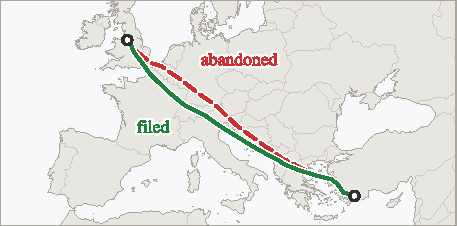
\includegraphics{fig_example_map.pdf}\\[2mm]
\footnotesize
\setlength{\tabcolsep}{5pt}
\begin{tabular}{@{}lrr@{}}
\toprule
 & \textit{abandoned} & \textit{filed} \\
\midrule
planned fuel [kg]       & 10\,485 & 8\,469 \\
flight time [min]       & 259     & 258 \\
route charges [EUR]     & 2\,269  & 2\,496 \\
\midrule
model score             & $-2.82$ & $+0.90$ \\
\bottomrule
\end{tabular}\\[2mm]
gap $= 3.7 \;\longrightarrow\; P = 0.99 \;>\; \tau = 0.600 \;\longrightarrow$ proposed
\caption{The worked example from the text, on an anonymised city pair.
The route initially on file (dashed red) and the fuel-saving
alternative (solid green) are shown. The alternative saves 2\,016\,kg
of planned fuel at 227\,EUR more in route charges and the same flight
time. The calibrated acceptance probability exceeds the threshold; the
airline's own later filing chose the proposed route.}
\label{fig:example}
\end{figure}

% Cut for space, 2026-09-09 (author's request: the paper is too long,
% cut model ageing entirely). Section "Model ageing" (labelled
% sec:horizon, tab:horizon, fig:horizon) removed in full: a
% retraining-horizon experiment fitting the same configuration on
% January-October 2025 and evaluating month by month through June
% 2026, finding pairwise accuracy U-shaped between 64.6\,\% (three
% months out) and 68.0\,\% (six months out), the channel's proposal
% precision holding inside a 77.2-78.9\,\% band throughout while its
% proposal volume fell from 22.2\,\% to 17.3\,\% of eligible flights
% (a season-matched comparison put the net cost of three months'
% staleness at 1.9 points of volume and 1.3 of precision), and a
% recommendation to retrain quarterly. The second, ageing-only data
% split it depended on is removed with it (was documented in
% Section~\ref{sec:splits}). Every cross-reference to this section, to
% the fourth introduction contribution it supported, and to the fifth
% Conclusions finding, is removed or reworded at the point it occurred.
% =====================================================================
\section{Threats to validity}
\label{sec:validity}

The limitations of this study are collected here rather than scattered,
in the order of how much they bound the claims.

\paragraph{The label is behaviour, not utility} A revision records what
the airline's filing process produced, folding together its
economics, its dispatching software, its habits and its workload; the
model learns this compound, arguably the right target for a proposal
channel, since a proposal is accepted or ignored by the same compound.
Two consequences follow. First, a revision need not be a choice at
all: a route that ceased to be filable has to be replaced whatever
the airline would have preferred, and the archive carries no field
that separates such a revision from a deliberate one, so a share of
the labels that cannot be quantified here records a constraint rather
than a preference. Second, nothing in this paper measures a
preference in the economic sense of \citet{samuelson1938} separately
from the process that expresses it, and transfers of the learned
function to settings where the process differs (e.g., another
region's filing culture) should be expected to degrade.

\paragraph{Flights that never revise} Every revision pair is a flight
that changed its plan, yet a channel used in practice would see every
flight, and most never revise, so the model would be asked a question on which
it was evaluated only through the small stay set of Section~\ref{sec:stay}.
Precision should be expected to fall there, though not for the reason
it is tempting to give: non-revision has several causes besides
contentment with the filed plan (nothing prompted a second look, the
dispatch desk had no capacity, the flight departed before a relevant
regulation was published), and the channel's premise, that the latter
two are common, is not measured here. What the stay pairs do close, as
Section~\ref{sec:changebias} shows, is the model's tendency to
recommend change against traffic that stays, from 34.8\,\% to 90.0\,\%,
and not by reading regulation status, since the model scores 88.0\,\%
on the population where that shortcut would be wrong. Two bounds
remain: the stay set is small (1\,093 test pairs) and its two routes
belong to different flights, so a model could learn the construction
rather than the preference it encodes, the one place in this paper
where a score compares routes across flights rather than within one.
A balanced stay dataset, matching same-flight routes with regulation
status independent of the label, requires data not currently
assembled and is the single most valuable extension of this work. The
never-revise limitation falls harder on the second use case of
Section~\ref{sec:usecases} than the first, since an overload release
ranks flights on the volume, most of which never revise, which is why
that use case is described as enabled rather than demonstrated.

\paragraph{The candidates would come from somewhere else} In this
simulation the alternative offered to a flight is the route the
airline was about to file; a channel used in practice has no such
route and would have to obtain candidates from a generator, precisely the
distribution Section~\ref{sec:pairsvsets} argues is a poor source of
\emph{labels}. The argument transfers uncomfortably to serving time:
a model trained on two routes that both passed an airline's own
flight-planning system may score a generated route low for reasons
that have nothing to do with preference, a gap nothing in this paper
measures, since every figure in Section~\ref{sec:channel} is
conditioned on a candidate the airline had itself produced. A first
trial should accordingly draw its candidates from routes that
operator has filed before on that city pair, where the concern does
not arise, rather than from a generator.

\paragraph{The route is carried as a vocabulary, not a geometry} The
waypoint sequence enters the model as a bag of published identifiers, so
the 1.4 points it is worth are knowledge of a particular vocabulary
rather than of route shape, and two limits follow. Those identifiers are
European, so a model fitted here would carry little of that knowledge to
another region, which is the same non-transferability that the first of
these limitations predicts for the filing process itself. They are also
revised from time to time as the route network is republished, so a piece
of airspace can reappear under a name the model has never met, with
nothing in the encoding to connect the two; such changes are infrequent,
and the effect is correspondingly slow, but it is a drift that only
retraining repairs. Section~\ref{sec:ablation-sec} reports the attempt
to replace the vocabulary with a learned representation of route
shape, and why it did not succeed; a representation that does not
depend on names would nonetheless be what makes the model portable,
and remains the most valuable direction on this axis.
% Added 2026-09-07 at the author's request; the encoder trial it points at
% was already reported in Section 6.3.

\paragraph{Fuel is not always a stable, burned cost} Two separate
issues limit every fuel figure in this paper. First, every figure
rests on planned fuel, which differs from burned fuel by whatever the
tactical phase imposes (e.g., a direct routing granted en route, or a
cruise level capped below the one requested); quantifying that
difference requires flown trajectories matched to the plans that
preceded them, and until that is done the totals of
Section~\ref{sec:channel} should be read as an upper bound on what a
proposal channel would deliver. Second, planned fuel enters the model
in kilogrammes and route charges in euros, two units that move on
independent schedules: a kilogramme of jet fuel bought in 2025 is not
the same expense as one bought in 2035, so any trade-off the model has
learned between the two reflects the archive's own prices rather than
a stable preference, though nothing in eighteen months of training
data teaches the model that this relationship drifts, because within
that window it barely does. Recasting fuel as a monetary cost before
training, or normalising every indicator to a common unit, would make
the learned trade-offs portable across the years a model like this one
would remain in use.

\paragraph{The counterfactual is absent} On every flight the simulation
counts, the airline found the cheaper route by itself, so the 20.1\,kt
is not fuel that a channel would create but fuel that a channel could
have surfaced earlier. What a channel would genuinely add, the flights
on which the alternative was never considered, is precisely what this
data cannot measure, and only a trial with real proposals and logged
acceptance can close this gap and observe acceptance itself rather
than its revealed proxy.

\paragraph{The regulation picture is the binding constraint at serving
time} Attributed delay and the regulation picture are among the
strongest inputs, and both are properties of a moment rather than of a
flight, so a score computed against a regulation state that has since
changed no longer describes the decision at hand: the binding
constraint at serving time is data currency rather than computation,
since the scoring step itself is a single pass through a fixed tree
ensemble. Harder, and unmeasured here, is that the alternative
route's attributed delay is known in the archive only because the
airline went on to file that route. For a route nobody has filed, the
delay it would attract is
a query rather than an observation, and the error in answering it would
propagate into the acceptance probability.

% =====================================================================
\section{Conclusions}
\label{sec:conclusions}

Airline route acceptance is learnable from flight-plan revisions at
network scale, and the findings of this paper are fourfold. First, a
model fitted on 1\,134\,000 revisions identifies the chosen route in
68.1\,\% of held-out cases and supports operation at a selected
precision rather than at a single accuracy figure: on the most
confident fifth of the decisions it is right 94.9\,\% of the time.
% Cut for space and for political sensitivity, 2026-09-08 (matching the
% SID redaction): previously "every rule preferring the route that is
% cheaper on one of the four planning indicators scores below chance on
% this archive, so that the strongest simple rule is an inverted one at
% 55.0\,\%, and". The legitimate finding that follows it, that the
% model's advantage concentrates where cost logic fails, is kept; only
% the inverted-rule framing that led into it is removed.
Secondly, no single cost indicator predicts the choice well on this
archive, the strongest such rule reaching only 55.0\,\%. Thirdly, a proposal channel tuned for 80\,\% precision and delivering
79.2\,\% addresses 20.1\,kt of planned fuel per quarter, validated against what
the airlines subsequently filed, four fifths of it flown by 28 of 882
operators, and these figures are robust to the stay-pair bias
correction. Fourthly, route structure carries information about
the choice that the cost indicators do not: the waypoint sequence is
the largest single term in what moves the model's score, though the
cost indicators together outweigh it and removing the sequence costs
only 1.4 points of accuracy.

A route
that burns less planned fuel emits less carbon dioxide, and the reason
such routes go unflown is not that nobody can find them but that nobody
knows which of them an airline would actually take. That is the gap
this paper addresses, and the reason acceptance rather than fuel is the
quantity modelled: a proposal an airline declines saves nothing, and a
channel that makes many of them is switched off. Ranking candidate
routes by likely acceptance is what allows the environmentally cheaper
proposals to be aimed at the flights on which they are also cheap for
the operator, which is the only version of this idea that both sides
have a reason to run.

The number that characterises this system is not 68.1\,\% but the curve
of Fig.~\ref{fig:coverage}, because a channel chooses where on that
curve to sit, and because ranking a pair correctly and proposing
correctly are different quantities of which the second is the
operational one: at the threshold used here, the channel proposes on about a fifth
of the eligible flights, and 79.2\,\% of those proposals match what the
airline went on to file. Were such a channel ever used, it would sit
well to the left of that curve, moving right only as acceptance is
observed. The second use case of Section~\ref{sec:usecases},
choosing which flights to ask to reroute when a volume of airspace is
overloaded and in which order, remains enabled rather than
demonstrated: it needs the same acceptance probability, on a
population this archive cannot speak for.

% CORRECTED 2026-09-09 (author's request: keep the framing to
% research, not an implied operational trial). The proposal to "run a
% shadow-mode trial logging the real responses of airlines... the
% first turn of the feedback loop" is removed; the open question it
% named (observing acceptance directly rather than through its
% revealed proxy) is kept as a research question.
Future work should assemble a balanced stay dataset in which
regulation status is independent of the label, which is what
currently bounds the change-bias measurement, and match flown
trajectories to the plans that preceded them, so that planned savings
can be restated as burned ones. Observing acceptance directly, rather
than through the revealed proxy this paper relies on, remains an open
question beyond its scope.

% Cut for space, 2026-09-09 (author's request: cut model ageing
% entirely). This paragraph previously opened by crediting "the
% horizon experiment of Section~\ref{sec:horizon}" with giving a
% deployment plan its retraining cadence; the clause is removed with
% the section, the remaining point kept.
Only a live channel can reveal how preferences shift once proposals
themselves begin to influence filing behaviour, so any practical use
of this model would need to re-measure everything this paper
measures.

\section*{Disclaimer}
The views expressed are those of the authors and do not necessarily
reflect the official position of EUROCONTROL or of its Member States.
This paper reports research and does not commit to any operational
service.

% NOTE: the role assignment below is INFERRED from author order and
% affiliations (first author = modelling and drafting; MUAC authors =
% operational domain, data and validation; Innovation Hub senior
% author = project administration; HQ authors = supervision). Every
% author must confirm or correct their roles before submission.
\section*{CRediT authorship contribution statement}
\textbf{Ramon Dalmau:} Conceptualization, Methodology, Software, Data
curation, Formal analysis, Investigation, Visualization, Writing --
original draft. \textbf{David Perez:} Conceptualization, Resources,
Validation, Writing -- review \& editing. \textbf{Franck Ballerini:}
Validation, Writing -- review \& editing. \textbf{Seddik Belkoura:}
Methodology, Validation, Writing -- review \& editing.
\textbf{Vincent Taverniers:} Resources, Data curation, Writing --
review \& editing. \textbf{Gratiel Marius Marin:} Resources,
Validation, Writing -- review \& editing. \textbf{Robin Deransy:} Conceptualization, Project
administration, Writing -- review \& editing. \textbf{Benjamin
Cramet:} Supervision, Writing -- review \& editing. \textbf{Grigori
Gustin:} Supervision, Project administration, Writing -- review \&
editing.

\section*{Declaration of generative AI and AI-assisted technologies in
the writing process}
% Cut for space, 2026-09-09 (author's request: the paper is too long,
% and the figure this disclosure concerned, Fig.~\ref{fig:method}, was
% itself cut). The paragraph previously disclosed Google's Gemini image
% model as having produced that figure, a methodology schematic, and
% gave the publisher-facing detail its use required (no data or result
% in the figure beyond dataset sizes and settings stated in the text;
% generated under the authors' direction; every label checked; two
% corrected by hand; the authors deferring to the editor on whether a
% manually drawn equivalent was required). None of that applies once
% the figure is gone. What remains true and is kept below: Claude was
% used for text and for the analysis figures, and no figure was
% created or altered with generative AI.
During the preparation of this work the authors used Claude
(Anthropic) to assist with drafting and editing the manuscript text
and with producing the analysis figures from the study's result
tables. Every analysis figure is drawn by the authors' own code from
the study's result tables, and no figure in this paper was created or
altered with generative AI. After using these tools, the authors
reviewed and edited the content as needed and take full responsibility
for the content of the published article.

\section*{Declaration of competing interest}
The authors declare that they have no known competing financial
interests or personal relationships that could have appeared to
influence the work reported in this paper.

\section*{Data availability}
The data used in this study is operational air traffic data held by
EUROCONTROL and processed under existing data-handling arrangements; it
cannot be made publicly available. Aggregated tables underlying every
figure are available from the corresponding author upon reasonable
request, in the de-identified form this paper itself uses: operators,
city pairs and waypoints appear in them by rank rather than by name,
which leaves every number and every ordering unchanged. Tables holding
one row per flight are not part of that offer.

\bibliographystyle{elsarticle-harv}
\bibliography{refs}

\end{document}
